\documentclass[10pt]{article}
\setlength\parindent{0pt}

\usepackage[english]{babel}
\usepackage[utf8x]{inputenc}
\usepackage{amsmath}
\usepackage{graphicx}
\usepackage{amssymb}
\usepackage{subcaption}
\usepackage[margin=0.5in]{geometry}
\usepackage{float}

\title{Pattern Classification and Machine Learning\\Mini Project Report}
\author{Erol Can Ün, Ferhat Elmas}

\begin{document}
\maketitle

\section{Introduction}
The aim of this project is to understand several supervised machine learning algorithms (multilayer-perceptron (MLP), linear classifiers with squared and logistic error functions) via implementing them in the context of a subset of a real world computer vision problem; namely, object recognition. NORB 3D dataset consisting of the photos of objects of different types, i.e. four legged animals, humans, airplanes, trucks and cars, taken by two cameras from left and right, is used for classification. Dataset is composed of 10800 pictures which are divided equally for training and testing. Firstly, a MLP for binary  classification is implemented in MATLAB to classify images from the NORB dataset. Then, its machinery is updated to a multi-class MLP to classify five targets. Moreover, linear classifiers with squared error function enhanced by a Tikhonov regularizer and a logistic error function are implemented.

\section{Methods}
\subsection{Binary Classification}
A binary classifier which uses a MLP with two hidden layers and a logistic error function was implemented. The structure of the network is as in the project description.

\subsubsection{Data Preprocessing}
Preprocessing does not deviate from the method given in the project instructions. Both training and test dataset is composed of data matrices for left and right cameras, with pixels serialized column-wise for each sample in the dataset. Data is originally stored in uint8 format so we converted it to double number format before operating on it. After splitting the dataset given for training into training and validation datasets with a ratio of 2/3 and 1/3 respectively, normalization was applied. This was accomplished by calculating the mean and standard deviation across the training set and then subtracting their individual means and multiplying with multiplicative inverse of standard deviation for every pixel(feature). This was then repeated for validation set and test set, but with means and standard deviation calculated for the training set only. Target values were also mapped from \{1,3\} to \{-1,1\}. Note that test set was not used in any part of training.

\subsubsection{Training and Model Parameter Selection}
After implementation, we trained our MLP with the training and validation datasets, explicitly reserved for early-stopping. We had four parameters that could be modified: number of hidden nodes in first and second layers of MLP (h1 and h2), learning rate and momentum of gradient descent algorithm, which is used together with back-propogation to update weight and bias gradients as described in the course notes. Our training methodology was as follows: We first tried three different combinations of h1 and h2 to observe the performance of the network with respect to those parameters. 

We employed early-stopping, which suggests stopping training after validation error starts increasing. After some experimentation, we observed that stopping training as soon as validation error starts increasing is \textit{not} a good practice since validation error was not very stable in the first few epochs. Therefore, we stopped training as soon as we had three validation errors in a row that had the same or very close values defined by a very small difference threshold. Zero-one error for the validation set was not used to that purpose since it remained zero throughout the training. We later calculated logistic and zero-one errors for the test set with those parameters. 

Similarly, we fixed h1 and h2 to values that provided the best performance in the first part in terms of convergence speed and overfitting, and used three different combinations of learning rate and momentum to train the models using early-stopping.

\subsubsection{Testing the Model}
After having tried different combinations of hidden units, learning rate, momentum, we fixed all of them to train a final network to be used on test set. We trained the network with different weight initializations to see how network reacts to different initializations. Later, we decided on an initialization and tested our network with test dataset.

\subsection{Multi-way Classification}

\subsubsection{Data Preprocessing}
Preprocessing is the same as in binary. However, for linear regression, splitting and normalization were done for each trial of cross validation individually. Then, a general normalization was applied to training and test sets to calculate the optimum weights.

\subsubsection{Linear Regression with Squared Error}
We firstly encode each class target as a vector. It is constructed as a zero vector of length equal to number of targets and then index corresponding to assigned target is set to one. If the target $t_i$ is 3, it will be represented as $\tilde{t_{i}}=[0, 0, 0, 1, 0]$, where $t_i$ can take integer values between 0 and 4. Squared error is calculated as follows:

\begin{equation}\label{eq:sqrerr}E_{2}(W)=\frac{1}{2}\sum_{i=1}^N\left\Vert y_i - \tilde{t_i}\right\Vert^2 \end{equation}

The linear classifier calculates $y_i$ by $w_{k}^T\tilde{x_i}$ where $\tilde{x_i}$ is constructed by appending 1 as bias term to the original instance such that $\tilde{x_i}=[x_i; 1]$. This multiplication creates a vector of size of 5. Then, prediction target is found by $argmax_k y_i(k)$.

$W_{optimal}={(\Phi^T\Phi)}^{-1}\Phi^T \tilde{T}$ where $\Phi$ is the feature matrix ($n \times d$) that holds instances in its rows (which is just the data itself in our case) and $\tilde{T}$ is a matrix ($n \times k$) that holds corresponding encoded targets row-wise. According to our data, $n=5400, d=2\times576+1=1153$ and $k=5$. W is of size ($d \times k$), i.e. weight vectors for each sample concatenated column-wise.

\subsubsection{Improved Squared Error with Regularizer}
Ill-conditioning of the matrix in the normal equation in previous section is avoided using squared error with Tikhonov regularizer:

\begin{equation}\label{eq:reg_tik} E_{reg}(W)=E_2(W) + v \sum^K_{i=1}{\left\Vert w_i \right\Vert}^2 \end{equation}

Corresponding optimum weights can be found by $W = (\Phi^T\Phi + vI)^{-1}\Phi^T \tilde{T}$. This modification increases test error on the expense of dealing with an ill-conditioned matrix inverse in the normal equation. We used 10-fold cross validation to find the optimum $v$. Training set was splitted into 10 folds of equal number of samples and each fold was used in turn as a validation set whereas the remaining 90\% was used for training. For each value of $v$, we used normal equation with regularizer to calculate optimum W and use it to find validation error for each trial. Average validation error for given $v$ was calculated. In the end, the optimum $v$ that resulted in the minimum validation error among others was used to train the model with whole training set. $\{0\} \bigcup \{c \times 10^i | i \in [0, 19], c=10^{-16} \}$ is the set of Tikhonov parameters used in cross-validation.

\subsubsection{Logistic Regression}

Squared error assigns a huge error to the outliers of the data and therefore not stable against small changes in the dataset. To combat this, logistic error function is utilized for linear classification:

\begin{equation}\label{eq:logerr}E_{log}(W)=\sum^N_{i=1} \text{lsexp}(y(x_i)) - \tilde{t_i^T} y(x_i)\end{equation}

Since there is no analytical solution to find the weight that minimizes this error function, gradient descent is applied to the gradient of error function:

\begin{equation}\nabla_{W} E = (\sigma(Y) - \tilde{T}^T) \times X^T\end{equation}

where $\sigma(Y) = [\sigma(y_i)], \tilde{T}^T = [\tilde{t_i}]$ and $X = [x_i]$ with a row vector of 1 appended to account for bias vectors. For early stopping, the same method in binary classification is used, but this time with zero-one validation error. 

\subsubsection{Multi-Class MLP}

Different from binary MLP, we had 5 classes and squared error function instead of logistic. Since we had binary MLP at hand, we could extend it easily to a multi-class by only updating the residual of the last layer and increasing number of output nodes to five. It also meant we could use all forward calculations for binary case. Moreover, target class is encoded as in Section 2.2.2. Exactly the same methodology for the binary case was used for preprocessing and training.

\section{Results \& Discussion}

\subsection{Binary MLP}

\begin{table}[H]
\def\arraystretch{1.1}
\small
\center
    \begin{tabular}{| c | c | c | c | c | c | c |}
    \hline
    Figure.Trial & h1 & h2 & Learning Rate & Momentum & Initialization & Test Error \\ \hline \hline
    2.1 &10 & 90 & 0.1 & 0.9 & $\sim \mathcal{N} (0,1/n)$ & 0.0849  \\ \hline
    2.2 & 90 & 10 & 0.1 & 0.9 & $\sim \mathcal{N} (0,1/n)$ & 0.0640 \\ \hline
    2.3 & 50 & 50 & 0.1 & 0.9 & $\sim \mathcal{N} (0,1/n)$ & 0.0475 \\ \hline
    3.1 & 50 & 50 & 0.1 & 0.1 & $\sim \mathcal{N} (0,1/n)$ & 0.0850\\ \hline
    3.2 & 50 & 50 & 0.1 & 0.9 & $\sim \mathcal{N} (0,1/n)$ & 0.1167 \\ \hline
    3.3 & 50 & 50 & 0.9 & 0.9 & $\sim \mathcal{N} (0,1/n)$ & NaN  \\ \hline 
    4.1 & 50 & 50 & 0.1 & 0.1 & 1 & 0.7005 \\ \hline
    4.2 & 50 & 50 & 0.1 & 0.1 & 0.1 & 0.6934\\ \hline
    4.3 & 50 & 50 & 0.1 & 0.1 & $\sim \mathcal{N} (0,1/n)$ & 0.0808 \\ 
    \hline
    \end{tabular}
    \caption{Training parameters for binary MLP (n is number of inputs for corresponding weight/bias parameters}
    \label{parameters_binary}
\end{table}

\textbf{h1 \& h2:} First, we fixed learning rate and momentum to values suggested as optimum in the literature\footnote{http://www.willamette.edu/~gorr/classes/cs449/momrate.html} and trained our network with several h1 and h2. Please refer to Table \ref{parameters_binary} for training trials. As seen in Figure \ref{binary_h1h2}, low h1 and high h2 is the slowest in terms of convergence speed, whereas high h1 and low h2, is faster. Keeping number of nodes in each layer closer to each other performs between two extremes. For binary case, we might conclude that low h1 and h2 parameters do not affect training badly since number of features to be captured in a dataset with two targets is limited. On the other hand, increasing both saves from training time on the expense of increasing network complexity.

$\boldsymbol{\eta}$ \textbf{\&} $\boldsymbol{\mu:}$ Second, we fixed h1 and h2 to 50 since these were the optimum values from previous experiment in terms of convergence speed and final validation error. In Figure \ref{binary_numu}, when we keep learning rate low and change momentum from low to high, we cannot see much difference in convergence speed. If momentum is kept the same and learning rate is increased, there is no convergence. This might be due to gradient descent, making big oscillations around the optimum solution but failing to reach it. That is why small learning rate is vital to converge but since classes are easily separable, increase in momentum does not make much difference. It was difficult to observe overfitting for the binary case since validation error followed closely to the training error most of the time and zero-one error was always equal to zero. However, an increase in test error suggests some network configurations experience more overfitting, even though test error should never be used to select network parameters.

\textbf{Initialization:} Finally, we kept the optimum parameters of two previous experiments to see what different initialization methods bring in. From Figure \ref{binary_weights}, when all weights and biases are set to 1, gradient descent did not converge. When we decreased 1 to 0.1, it converged but took more time compared to $\mathcal{N}(0, 1/n)$, where $n$ is the number of input nodes. This helped us conclude that an initialization with too large weights put gradient descent far from a minimum optimum solution. There is also a possibility that it might be getting stuck at a local minimum instead of the global one.

\begin{figure}[H]

\includegraphics[keepaspectratio]{most_least_errored.png}
\centering
\caption{A sample of NORB image from the test set with most(left) and least(right) errored classification}
\label{most_least_errored}
\end{figure}

We display in Figure \ref{most_least_errored}, most and least errored images from the test set that are misclassified by our final model with the decided parameters. Both images are assigned the same target originally. We might deduce that lightning of the images reduces the accuracy of classification. Also, one could say that images that belong to this target with more lightning are scarce in the training dataset, therefore resulting in high error rates when they show up in the test set. This is also an example of overfitting: MLP adapts well to a training set of such targets with less lightning and therefore is not stable with unseen data that contains images from that target with more lightning.

\begin{figure}[H]
\centering
\begin{minipage}{.48\linewidth}
  \centering
  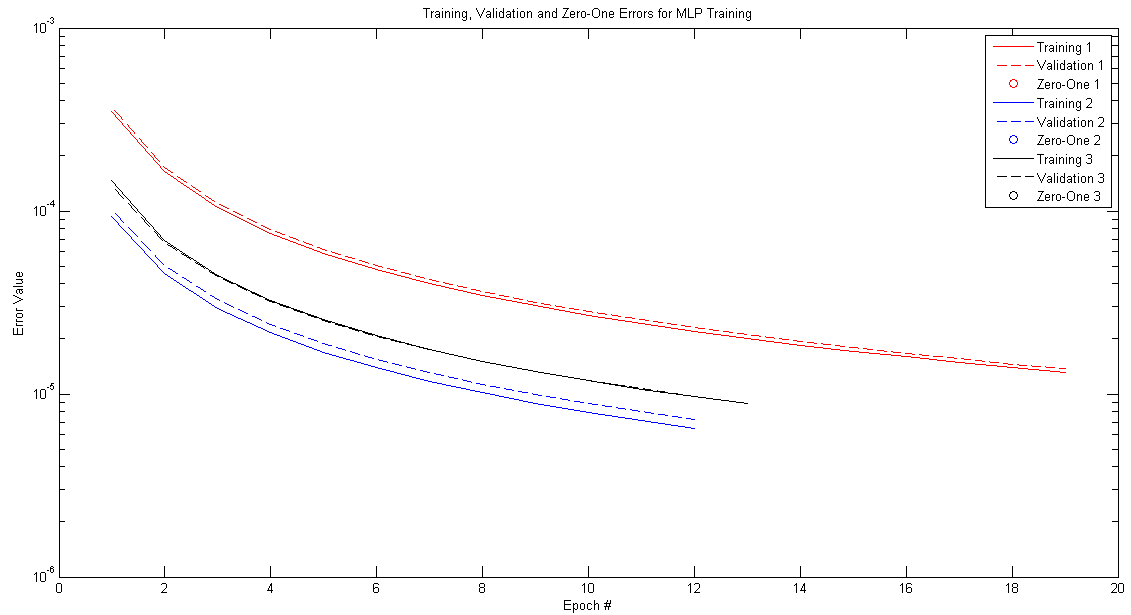
\includegraphics[width=\textwidth]{binary_h1h2.png}
  \captionof{figure}{Binary MLP training results with different number of hidden layer nodes}
  \label{binary_h1h2}
\end{minipage}
\hspace{.03\textwidth}%
\begin{minipage}{.48\linewidth}
  \centering
  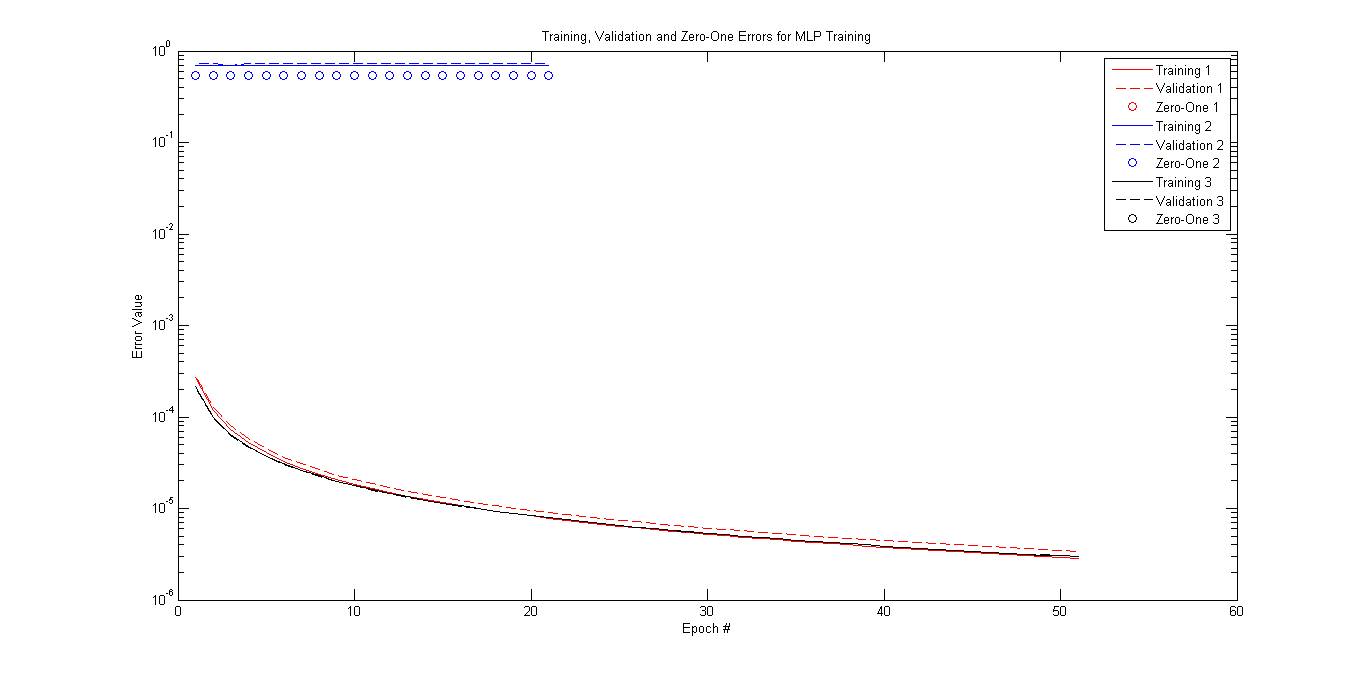
\includegraphics[width=\textwidth]{binary_numu.png}
  \captionof{figure}{Binary MLP training results with different learning rate and momentum values}
  \label{binary_numu}
\end{minipage}
\end{figure}

\begin{figure}[H]
\centering
\begin{minipage}{.48\textwidth}
  \centering
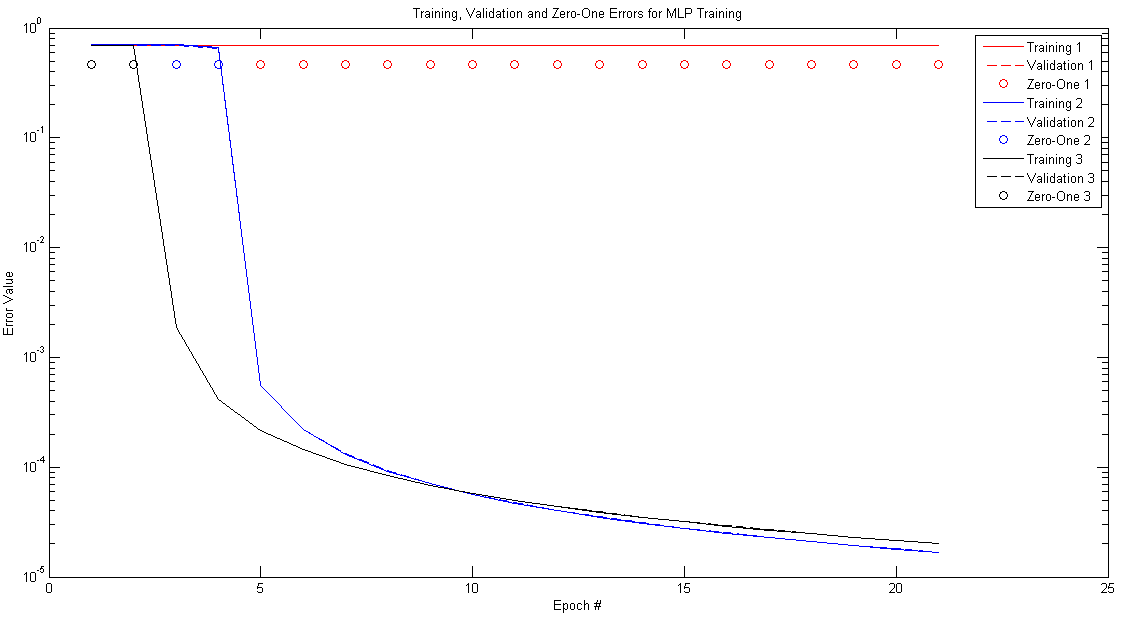
\includegraphics[width=\textwidth,height=\textheight,keepaspectratio]{binary_weights.png}
\captionof{figure}{Binary MLP training results with different weight initalizations}
\label{binary_weights}
\end{minipage}
\hspace{.03\textwidth}%
\begin{minipage}{.48\textwidth}
  \centering
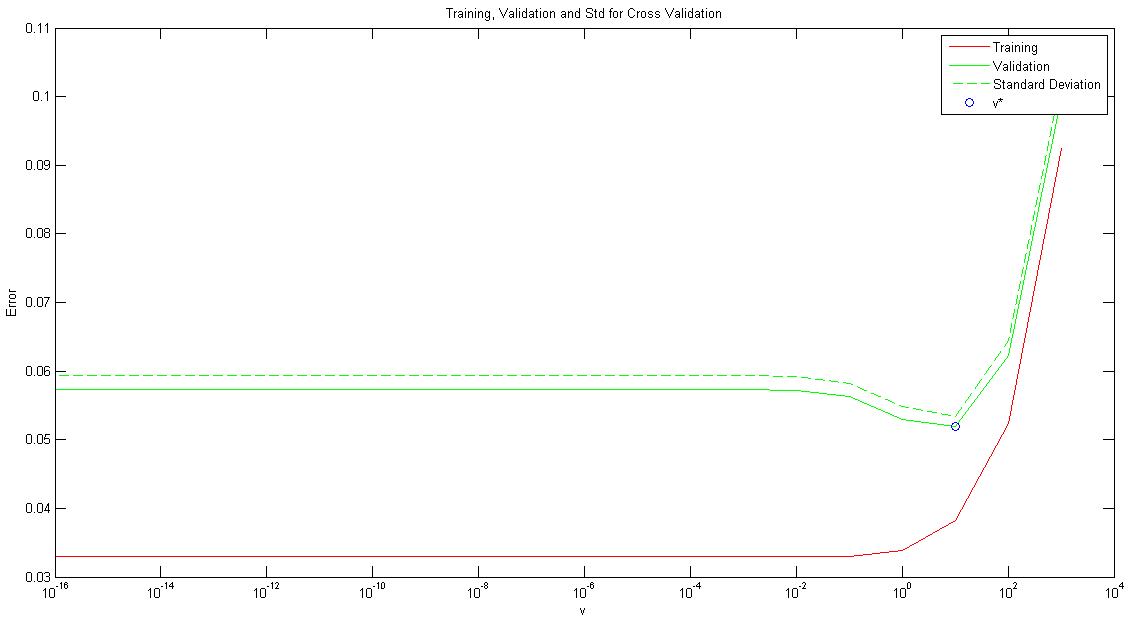
\includegraphics[width=\textwidth,height=\textheight,keepaspectratio]{cross_validation.png}
\captionof{figure}{Cross-validation for linear regression and optimum Tikhonov regularizer}
\label{cv}
\end{minipage}
\end{figure}

\subsection{Linear Regression with Tikhonov Regularization}
To find the best regularization parameter, we apply 10-fold cross validation. As seen in Figure \ref{cv}, we choose $v=10$ where the validation error is minimum. Bias-variance tradeoff comes into play with model parameter selection, where Tikhonov regularization parameter $v$ is the one to be selected. In the figure, bias of the model can be represented by the training error whereas average validation error represents the variance. Optimally, the point at which both are minimum is ideal for model selection. Having a smaller bias assures that model is more loyal to the underlying distribution of data whereas a minimum variance signifies the strong stability of model against unseen data. Dashed line is the mean of average validation error + standard deviation, which represents how much validation error deviates from the mean of expected test risk of our model, among folds, for each value of $v$. 

\subsection{Logistic Regression}

\begin{table}[H]
\def\arraystretch{1.1}
\small
\center
    \begin{tabular}{| c | c | c | c | c |}
    \hline
    Figure.Trial & Learning Rate & Momentum & Initialization & Test Error \\ \hline \hline
    6.1 & 0.1 & 0.1 & $\sim \mathcal{N} (0,1/n)$ & 0.7280  \\ \hline
    6.2 & 0.1 & 0.9 & $\sim \mathcal{N} (0,1/n)$ & 0.5471 \\ \hline
    6.3 & 0.9 & 0.9 & $\sim \mathcal{N} (0,1/n)$ & 1.4077 \\ \hline
    7.1 & 0.1 & 0.9 & $\sim \mathcal{N} (0,1/n)$ & 0.5623\\ \hline
    7.2 & 0.1 & 0.9 & $\sim \mathcal{N} (0,1/(100n))$ & 0.5963 \\ \hline
    7.3 & 0.1 & 0.9 & 0.1 & 0.5577  \\
    \hline
    \end{tabular}
    \caption{Training parameters for logistic regression (n is number of inputs for corresponding weight/bias parameters}
    \label{parameters_logistic}
\end{table}

$\boldsymbol{\eta}$ \textbf{\&} $\boldsymbol{\mu:}$ We applied gradient descent to solve for optimum W that minimizes logistic error function. From Figure \ref{logistic_numu}, the effect of learning rate and momentum is seen better compared to binary classification. If learning rate is kept the same, increasing momentum decreases convergence time (6.1 vs 6.2). While momentum is fixed, increasing learning rate also increases convergence speed (6.2 vs 6.3). With low momentum and low learning rate, the oscillations of steps are much more frequent but each contributes to a small change in error. In addition, change in one epoch has a higher slope. While momentum is increasing, curvature of error function gets smoother, which shows damping along the directions orthogonal to the optimum solution. Increasing learning rate increases the size of steps taken towards the optimum solution.

\textbf{Initialization:} From Figure \ref{logistic_weights}, we see similar trends for different initialization methods such as uniform or gaussian with different variances because logistic regression is not adversely affected by outliers like in linear regression: Variance among the inputs does not influence the optimum seperating hyperplane much. What is more, uniform weight initialization results in the lowest test error. This suggests that logistic regression with uniform weights helps dampen overfitting. 

\begin{figure}[H]
\centering
\begin{minipage}{.48\textwidth}
  \centering
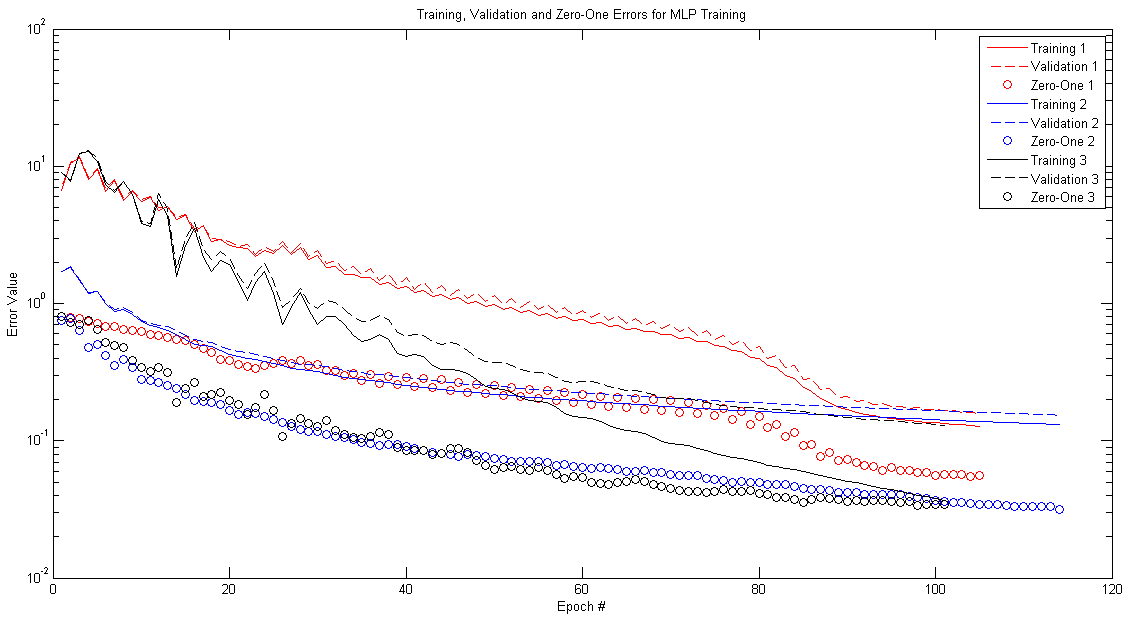
\includegraphics[width=\textwidth,height=\textheight,keepaspectratio]{logistic_numu.png}
\captionof{figure}{Logistic regression gradient descent results with different learning rate and momentum}
\label{logistic_numu}
\end{minipage}
\hspace{.03\textwidth}%
\begin{minipage}{.48\textwidth}
  \centering
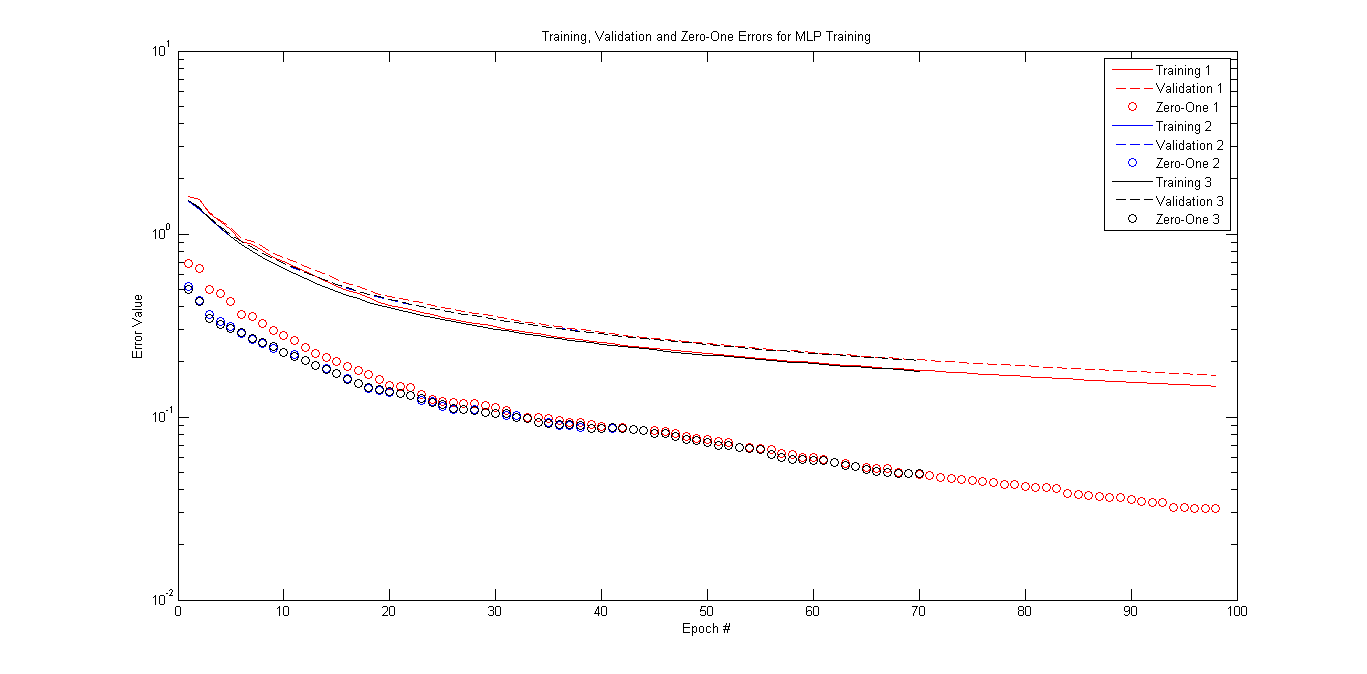
\includegraphics[width=\textwidth,height=\textheight,keepaspectratio]{logistic_weights.png}
\captionof{figure}{Logistic regression gradient descent results with different weight initalizations}
\label{logistic_weights}
\end{minipage}
\end{figure}

\subsection{Multi-class MLP}

\begin{table}[H]
\def\arraystretch{1.1}
\small
\center
    \begin{tabular}{| c | c | c | c | c | c | c |}
    \hline
    Figure.Trial & h1 & h2 & Learning Rate & Momentum & Initialization & Test Error \\ \hline \hline
    8.1 & 10 & 90 & 0.1 & 0.9 & $\sim \mathcal{N} (0,1/n)$ & 0.2380  \\ \hline
    8.2 & 90 & 10 & 0.1 & 0.9 & $\sim \mathcal{N} (0,1/n)$ & 0.4199 \\ \hline
    8.3 & 50 & 50 & 0.1 & 0.9 & $\sim \mathcal{N} (0,1/n)$ & 0.1371 \\ \hline
    9.1 & 50 & 50 & 0.1 & 0.1 & $\sim \mathcal{N} (0,1/n)$ & 0.1386\\ \hline
    9.2 & 50 & 50 & 0.1 & 0.9 & $\sim \mathcal{N} (0,1/n)$ & 0.1406 \\ \hline
    9.3 & 50 & 50 & 0.9 & 0.9 & $\sim \mathcal{N} (0,1/n)$ & NaN  \\ \hline
    10.1 & 50 & 50 & 0.1 & 0.9 & $\sim \mathcal{N} (0,1/n)$ & 0.1398 \\ \hline
    10.2 & 50 & 50 & 0.1 & 0.9 & $\sim \mathcal{N} (0,1/(2n))$ & 0.1322 \\\hline
    10.3 & 50 & 50 & 0.1 & 0.9 & $\sim \mathcal{N} (0,1/(100n))$ & 0.1281\\
    \hline
    \end{tabular}
    \caption{Training parameters for 5-class MLP (n is number of inputs for corresponding weight/bias parameters}
    \label{parameters_multi}
\end{table}

\textbf{h1 \& h2:} Refer to Figure \ref{multi_h1h2}. Network with low h1 and high h2 converges slower compared to the network with similar h1-h2 pair. This is likely due to network not being able to capture enough features of the data in the first layer and thus, resulting in an inefficiency with updating the weights during backpropogation. On the other hand, high h1 and low h2 does not converge to a minimum and gets stuck with a local minimum. This might suggest that network having more parameters to update in the first layer than it has on the second layer experiences problems in backpropogation. We might assume that propogation of residuals from a weaker second layer to a more complex first layer is not captured well by the network and therefore it is saturated with a local solution. Nevertheless, more complexity needs to be introduced since first layer needs to identify large amount of information coming from 5 different classes, that makes each distinctive. To compensate for this trade-off, having similar h1 and h2 both being in mid-range between 10 and 90 is satisfactory.

Notice also that overfitting is more dominant with Trial 2, as the gap between training and validation error widens in the figure. This is also evident with the higher test error obtained for that trial. As the amount of distinctive information about each class reduces with each layer, a dominance of number of such nodes in the first layer helps the network adapt fast to distinctive features in the training data but fails to capture new features introduced by test data.

$\boldsymbol{\eta}$ \textbf{\&} $\boldsymbol{\mu:}$ Similar to 2-MLP, high learning rate and momentum at the same time results in big steps that oscillate around the solution and therefore, error value for Trial 3 in Figure \ref{multi_numu} will not decrease. With little learning rate and momentum as in Trial 1, momentum is insiginificant and learning rate takes the lead. Convergence speed is similar for two trials but notice the increased overfit with low momentum. In addition, gradient updates are larger compared to that of 2-MLP. We think this is because of squared error function exaggerating large updates in the gradient. When using a momentum of 0.9, the effective learning rate can grow to 10 times the actual rate if the direction of weight changes is consistent. This is explained by the fast descent of error value for certain epochs in the figure.  

\textbf{Initialization:} After fixing all the parameters, weights with normal distribution with different variances were tested. One with the smallest variance was the fastest to converge. Higher variance does not improve zero-one and validation error and keeps doing a zig-zag update while improving training error. The smaller variance is, the less significant overfit becomes.

\begin{figure}[H]
\centering
\begin{minipage}{.48\textwidth}
  \centering
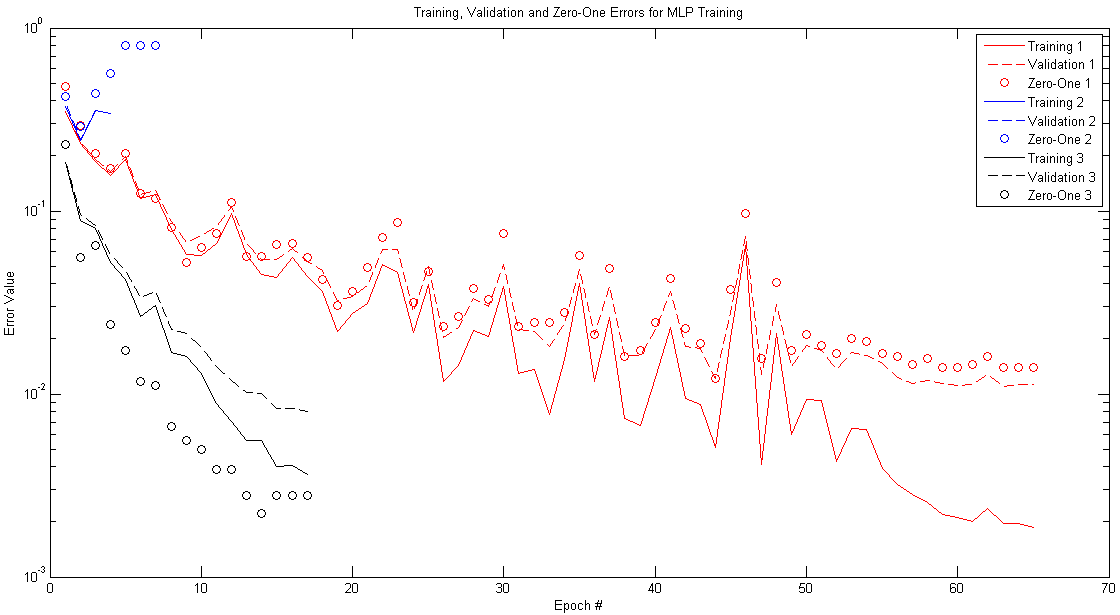
\includegraphics[width=\textwidth,height=\textheight,keepaspectratio]{multi_h1h2.png}
\captionof{figure}{5-way MLP training results with different number of hidden layer nodes}
\label{multi_h1h2}
\end{minipage}
\hspace{.03\textwidth}%
\begin{minipage}{.48\textwidth}
  \centering
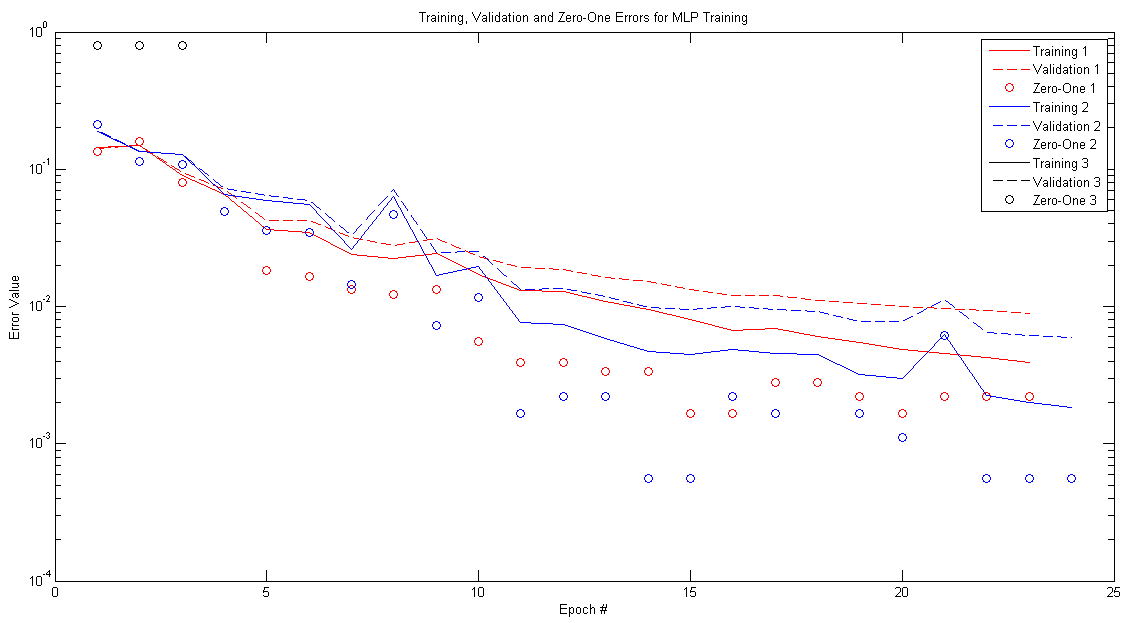
\includegraphics[width=\textwidth,height=\textheight,keepaspectratio]{multi_numu.png}
\captionof{figure}{5-way MLP training results with different learning rate and momentum values}
\label{multi_numu}
\end{minipage}
\end{figure}

\begin{figure}[H]
\centering
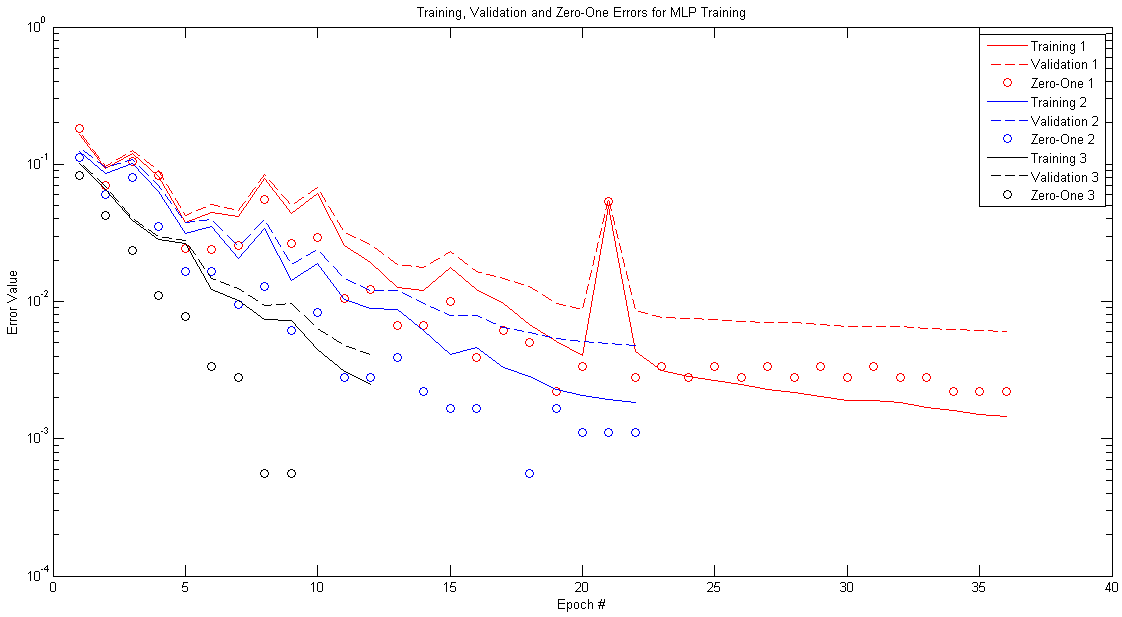
\includegraphics[keepaspectratio, scale = 0.32]{multi_weights.png}
\caption{5-way MLP training results with different weight initalizations}
\label{multi_weights}
\end{figure}

\subsection{Confusion Matrices and Final Models}

\begin{table}[H]
\def\arraystretch{1.1}
\small
\center
    \begin{tabular}{| c | c | c | c | c | c | c | c | c |}
    \hline
    Classifier & h1 & h2 & Learning Rate & Momentum & Initialization & Test Error & Zero-one Error & Std. Deviation \\ \hline \hline
    2-MLP & 50 & 50 & 0.1 & 0.1 & $\sim \mathcal{N} (0,1/n)$ & 0.0808 & 0.0244 & 0.0642  \\ \hline
    5-MLP & 50 & 50 & 0.1 & 0.9 & $\sim \mathcal{N} (0,1/(100n))$ & 0.1281 & 0.1894 & 0.0059 \\ \hline
    Linear & - & - & - & - & - & 0.4763 & 0.2054 & - \\ \hline
    Logistic & - & - & 0.1 & 0.9 & 0.1 & 0.5577 & 0.2106 & 0.0210 \\ \hline
    \end{tabular}
    \caption{Model parameters used for testing, test errors and standard deviation of test errors when initialized with three different weights as in Section 3}
    \label{test_results}
\end{table}

Table \ref{test_results} summarizes all parameters decided after training and test results. Standard deviation represents how each model behaves with three selected weight initializations as described in previous sections. It can be seen that 5-MLP is the one that is most stable against changes in initializations with a small standard deviation whereas 2-MLP is quite adaptive to different initial parameters. 

To compare, one might look at zero-one errors that give a neutral idea about the percentage of correctly classified instances in the test set. 5-MLP is the most accurate classifier for the multi-class classification, whereas linear and logistic regression show a similar performance. On the other hand, 2-MLP has the lowest error among all four, which suggests that decreasing complexity is open for more possibility of success. Nevertheless, we should note that training these models for classification is totally about parameter selection and with further optimization, different set of parameters for any of the classifiers could have resulted in a totally different test set performance.

\textbf{Confusion Matrices:} Objects used in classes are \textit{four-legged animals, humans, airplanes, trucks} and \textit{cars} for class labels 0, 1, 2, 3 and 4, respectively. \\

\begin{minipage}[b]{.30\textwidth}
  \centering
  \begin{tabular}{| c || c | c | c | c | c |}
    \hline
    Class & 0 & 1 & 2 & 3 & 4 \\ \hline \hline
    0 & 974 & 73 & 31 & 0 & 2  \\ \hline
    1 & 156 & 917 & 1 & 0 & 6 \\ \hline
    2 & 264 & 10 & 691 & 12 & 103 \\ \hline
    3 & 3 & 0 & 1 & 1038 & 38\\ \hline
    4 & 10 & 0 & 41 & 229 & 800 \\
    \hline
    \end{tabular}
    \captionof{table}{Confusion matrix for 5-class MLP}
    \label{confusion_mat_multi}
\end{minipage}\qquad
\begin{minipage}[b]{.30\textwidth}
  \centering
  \begin{tabular}{| c || c | c | c | c | c |}
    \hline
    Class & 0 & 1 & 2 & 3 & 4 \\ \hline \hline
    0 & 866 & 127 & 84 & 0 & 3  \\ \hline
    1 & 174 & 888 & 5 & 0 & 13 \\ \hline
    2 & 158 & 77 & 694 & 13 & 138 \\ \hline
    3 & 6 & 0 & 6 & 1015 & 53\\ \hline
    4 & 23 & 0 & 65 & 192 & 800 \\
    \hline
    \end{tabular}
    \captionof{table}{Confusion matrix for logistic regression}
    \label{confusion_mat_logistic}
\end{minipage}\qquad
\begin{minipage}[b]{.30\textwidth}
  \centering
\begin{tabular}{| c || c | c | c | c | c |}
    \hline
    Class & 0 & 1 & 2 & 3 & 4 \\ \hline \hline
    0 & 901 & 67 & 76 & 4 & 32  \\ \hline
    1 & 306 & 751 & 2 & 0 & 21 \\ \hline
    2 & 93 & 21 & 737 & 117 & 112 \\ \hline
    3 & 8 & 0 & 20 & 1036 & 16\\ \hline
    4 & 6 & 0 & 17 & 191 & 866 \\
    \hline
    \end{tabular}
    \captionof{table}{Confusion matrix for linear regression}
    \label{confusion_mat_linear}
\end{minipage}

Above confusion matrices can be used to interpret how each multi-class classifier treats each target individually. For example, in Table \ref{confusion_mat_multi}, diagonal entries \{i,i\} tells us how many instances in class $i$ are correctly classified whereas index \{3,1\} shows that none of the instances in class 3(trucks) were classified wrongly as 1(humans).

In practice, confusion tables provide us with extra evaluation measures for accuracy of the classifiers, besides zero-one error and others. For example, one could deduce that classes 3 and 4 are least confused with classes 0 and 1, which indicates that they have more distinctive features that separate them. Numbers being close to zero for indices \{i,j\}, where i,j = \{0,1,3,4\} confirms this. Contextually, this suggests four-legged animals and humans are least confused with trucks and cars. This could be due to many reasons, one of which is the distinctive shapes of such objects. Similarly, one could also notice that classes 0 and 1 are confused the most. This is not a big surprise because human figures look visually similar to four-legged animal figures. Thus, confusion matrices are also a good representation of perceptory and contextual understanding of data, especially if it consists of images.

One could also calculate \textit{True Positive} (TP) rate aka. \textit{Recall} for any class and for any classifier. It is the proportion of examples which were classified as class x, among all examples which truly have class x, i.e. how much part of the class was captured. In the confusion matrix, this is the diagonal element divided by the sum over the corresponding row. For our case, we could capture this by directly looking at diagonal entries since all classes have equal number of instances. It is evident that class 3 is the most successfully classified target for all 3 classifiers whereas the same thing cannot be said for target 2.

Another performance measure is the \textit{Precision}, which is the proportion of the samples which truly have class x among all those which were classified as class x. This is the diagonal element divided by the sum over the relevant column. For example, precision of class 3 for linear regression is $ 1036/(4+0+117+1036+191) = 0.7685$. This precision is much higher for logistic regression (0.832). We can also take the average of such measures for each class to obtain the average for each classifier and later use them to compare performance among classifiers. In the end, we could clearly induce that linear regression has difficulties capturing unique features of each target. Additional quantities such as \textit{False Positive} rate (FP) also exist in the literature. 

\subsection{Conclusion}
We were able to implement and train a MLP for multi-way classification. We achieved around 81\% accuracy on average, which is lower than the state-of-art result but that is not much bad performance. Overall, this is only a measure for the specific NORB dataset and parameters that we have been working on, and one could come up with many other configurations to increase this performance. The project helped us to learn and exercise tricky parts of training MLP. We also had a chance to evaluate performances of linear and logistic regression and make a comparison among all. Binary classification was the starting point and it helped us see how a network can be easily modified and upgraded to adjust it to different error measures with gradient descent and different network structures. Even though we calculated test error for all parameter combinations to make experiments, we strongly emphasize that test error should never be used during training in practice.

There are several optimizations and improvements for future work. The main aim of this project was to have an understanding of different classification methods for binary and multi-classes. For that reason, we have here a limited set of parameters for each algorithm. On the other hand, machine learning is more about trial and error in real world. In practice, it is recommended to try many more parameters to train the models and different algorithms to find the most optimized one for a given training dataset. Adaptive learning rate in gradient descent is one of the many recommendations. Model selection is also an important process, which could be accomplished with many different number of folds for cross validation, not to mention other algorithms for model selection. In the end, one should not be discouraged if one classifier does not perform well because there will be another one out there that is more suited to the data. All one needs to do is adjust network parameters sensibly and obtain a classifier that is robust to unseen test data.

\end{document}
